%%%%%%%%%%%%%%%%%%%%%%
%%%%%%%%%%%%%%%%%%%%%%
\section{Results}
%%%%%%%%%%%%%%%%%%%%%%
%%%%%%%%%%%%%%%%%%%%%%

\subsection{Performance of individual properties}
%%%%%%%%%%%%%%%%%%%%%%
%%%%%%%%%%%%%%%%%%%%%%
\subsubsection{SCOP fold}
%%%%%%%%%%%%%%%%%%%%%%
%%%%%%%%%%%%%%%%%%%%%%

\Cref{tab:vqscopt} shows the performance of each property when predicting SCOP folds.  Among structure-based properties we found that $\kappa$ backbone angles had the best performance, both for individual SCOP folds and in terms of its $AUC^{\bf{w}}$ ($0.961$).  Solvent accessibility (SolAcc) values performed the worst out of structure-based properties, obtaining the lowest $AUC$ for all SCOP folds and in terms of $AUC^{\bf{w}}$ ($0.868$). 

In general all structure-based properties outperformed sequence-based properties.  Among sequence-based properties predicted secondary structures performed the best, especially predictions that a residue is in a helix ($AUC^{\bf{w}}=0.788$), a loop ($AUC^{\bf{w}}=0.771$), or a sheet ($AUC^{\bf{w}}=0.787$).  Calculated hydrophobicity and VSL2B based predictions of disorder propensity performed the worst ($AUC^{\bf{w}}=0.707$ and $AUC^{\bf{w}}=0.682$ respectively).  As a predictor of disorder PDBDisorder-based features performed better than VSL2B ($AUC^{\bf{w}}=0.764$), although this may be based on information leak due to this predictor being trained on PDB data.

 %% TABLE
%%%%%%%%%%%%%%%%%%%%%
%%%%%%%%%%%%%%%%%%%%%
\begin{table*}[h]
\resizebox{\columnwidth}{!}{
	\begin{tabular}{|l||rrc|rrc|rrc|rrc||rrc||}
		\hline
		\multirow{2}{*}{Property\textbackslash Category} & \multicolumn{3}{c|}{All $\alpha$}& \multicolumn{3}{c|}{All $\beta$}& \multicolumn{3}{c|}{$\alpha/\beta$}& \multicolumn{3}{c||}{$\alpha+\beta$} & \multicolumn{3}{c||}{$AUC^{\bf{w}}$}\\ 
		\cline{2-16}
		 & $m$ & $n$ & $AUC$ & $m$ & $n$ & $AUC$ & $m$ & $n$ & $AUC$ & $m$ & $n$ & $AUC$ & $m$ & $n$ & $AUC^{\bf{w}}$\\
		\hline
		\hline
		Alpha & 4,096 & 8 & 0.994& 4,096 & 8 & 0.982& 4,096 & 16 & 0.967 & 4,096 & 32 & 0.829 & 4,096 & 8 & 0.930\\
		Kappa & 4,096 & 16 & 0.995& 4,096 & 16 & 0.986& 4,096 & 16 & 0.978 & 4,096 & 32 & 0.903 & 4,096 & 32 & 0.961\\
		Phi & 4,096 & 16 & 0.990& 4,096 & 16 & 0.975& 4,096 & 16 & 0.964 & 4,096 & 32 & 0.809 & 4,096 & 32 & 0.920\\
		Psi & 4,096 & 8 & 0.991& 4,096 & 16 & 0.981& 4,096 & 16 & 0.970 & 4,096 & 32 & 0.850 & 4,096 & 32 & 0.938\\
		SolAcc & 4,096 & 8 & 0.960& 4,096 & 8 & 0.951& 4,096 & 32 & 0.914 & 4,096 & 32 & 0.710 & 4,096 & 32 & 0.868\\
		\hline
		\hline
		B-factors & 256 & 8 & 0.790& 256 & 8 & 0.709& 64 & 8 & 0.809 & 16 & 4 & 0.587 & 64 & 4 & 0.717\\
		Helix & 16 & 4 & 0.868& 16 & 8 & 0.871& 64 & 16 & 0.842 & 64 & 32 & 0.637 & 64 & 32 & 0.788\\
		Hydrophobicity & 256 & 4 & 0.711& 1,024 & 4 & 0.728& 64 & 2 & 0.834 & 64 & 2 & 0.585 & 256 & 4 & 0.707\\
		Loop & 256 & 16 & 0.872& 64 & 8 & 0.848& 16 & 32 & 0.821 & 1,024 & 32 & 0.607 & 64 & 16 & 0.771\\
		PDBDisorder & 1,024 & 8 & 0.842& 64 & 4 & 0.849& 64 & 4 & 0.819 & 256 & 32 & 0.591 & 64 & 4 & 0.764\\
		Sheet & 64 & 2 & 0.904& 64 & 8 & 0.853& 256 & 16 & 0.836 & 64 & 32 & 0.641 & 64 & 32 & 0.787\\
		VSL2B & 16 & 2 & 0.699& 64 & 32 & 0.628& 64 & 8 & 0.812 & 64 & 2 & 0.589 & 64 & 8 & 0.682\\
		\hline
		\hline
		String Kernel & -- & 2 & 0.863& -- & 3 & 0.878& -- & 4 & 0.860& -- & 5 & 0.634 & -- & 4 & 0.794\\
		Sequence  & 64 & 16 & 0.915 & 64 & 16 & 0.876 & 64 & 16 & 0.880 & 64 & 16 & 0.621 & 64 & 16 & 0.813\\
		Structure & 4,096 & 32 & 0.992 & 4,096 & 32 & 0.983 & 4,096 & 32 & 0.979 & 4,096 & 32 & 0.903 & 4,096 & 32 & 0.961\\
		Sequence + Structure & -- & -- & 0.989 & -- & -- & 0.967 & -- & -- & 0.970 & -- & -- & 0.851 & -- & -- & 0.939\\
		Sequence + Structure + SK & -- & -- & 0.989 & -- & -- & 0.967 & -- & -- & 0.970 & -- & -- & 0.851 & -- & -- & 0.939\\

		\hline
		
	\end{tabular}
}
\caption[Optimal property based feature performance when predicting SCOP fold.]{Optimal performance, according to $AUC$, of each property based feature when predicting SCOP fold.  For each property feature the combination of $m$ and $n$ values that obtained the highest $AUC$ for an individual SCOP fold are reported.  The last three columns show the weighted $AUC$, $AUC^{\bf{w}}$, obtained across all SCOP folds. Results when combining all sequence and property based features are shown in the bottom section of the table.  Because different combinations of $m$ and $n$ are used when combining properties these values are not shown for the Sequence + Structure and Sequence + Structure + SK combination of features.}
\label{tab:vqscopt}
\end{table*}

%%%%%%%%%%%%%%%%%%%%%
%%%%%%%%%%%%%%%%%%%%%

%%%%%%%%%%%%%%%%%%%%%%
%%%%%%%%%%%%%%%%%%%%%%
\subsubsection{Catalytic activity}
%%%%%%%%%%%%%%%%%%%%%%
%%%%%%%%%%%%%%%%%%%%%%
The first column of results in \Cref{tab:vqgot} shows the performance of each property when predicting whether a protein is annotated with the catalytic activity term.  We found that disorder-based predictions (VSL2B  $AUC=0.742$ and PDBDisorder $AUC=0.718$) and predicted B-factors ($AUC=0.722$) performed the best, whereas, contrary to their performance in distinguishing between SCOP folds, predicted secondary structures performed the worst (Helix $AUC=0.687$, Loop $AUC=0.698$, and Sheet $AUC=0.681$).

%%%%%%%%%%%%%%%%%%%%%%
%%%%%%%%%%%%%%%%%%%%%%
\subsubsection{Catalytic activity subclass}
%%%%%%%%%%%%%%%%%%%%%%
%%%%%%%%%%%%%%%%%%%%%%
\Cref{tab:vqgot} shows the performance of each property when predicting the tested subclasses of catalytic activity.  As with predicting catalytic activity, predicted B-factors also performed well in predicting catalytic activity subclass ($AUC^{\bf{w}}=0.659$).  Predicted secondary structures had mixed performance, with predicted loops obtaining a comparatively high $AUC^{\bf{w}}$ of $0.647$, whereas helix and sheet predictions only achieved a $AUC^{\bf{w}}$ of $0.511$ and $0.621$ respectively.

%% TABLE
%%%%%%%%%%%%%%%%%%%%%%
%%%%%%%%%%%%%%%%%%%%%%
%\begin{centering}
%\begin{landscape}

%\begin{table*}[htbp]
\clearpage
\begin{sidewaystable}[H]

\vspace*{5in}
\begin{centering}
\resizebox{\textheight}{!}{




		\begin{tabular}{|l||rrc||rrc|rrc|rrc|rrc|rrc|rrc||rrc||}
		\hline
		\multirow{2}{*}{Property\textbackslash Category} & \multicolumn{3}{c||}{catalytic activity} & \multicolumn{3}{c|}{oxidoreductase activity}& \multicolumn{3}{c|}{transferase activity}& \multicolumn{3}{c|}{hydrolase activity}& \multicolumn{3}{c|}{lyase activity}& \multicolumn{3}{c|}{isomerase activity} & \multicolumn{3}{c||}{ligase activity} & \multicolumn{3}{c||}{$AUC^{\bf{w}}$} \\
		\cline{2-25}
		 & $m$ & $n$ & $AUC$ & $m$ & $n$ & $AUC$ & $m$ & $n$ & $AUC$ & $m$ & $n$ & $AUC$ & $m$ & $n$ & $AUC$ & $m$ & $n$ & $AUC$ & $m$ & $n$ & $AUC$ & $m$ & $n$ & $AUC^{\bf{w}}$\\
		\hline
		\hline
		B-factors & 256 & 32 & 0.722 & 4,096 & 32 & 0.709& 4,096 & 32 & 0.644& 4,096 & 32 & 0.630& 4,096 & 4 & 0.688& 4,096 & 32 & 0.738& 4,096 & 32 & 0.671 & -- & -- & 0.659\\
		Helix & 256 & 8 & 0.687 & 4,096 & 8 & 0.634& 4,096 & 32 & 0.603& 4,096 & 32 & 0.600& 4,096 & 32 & 0.644& 4,096 & 32 & 0.665& 4,096 & 8 & 0.595 & -- & -- & 0.611\\
		Hydrophobicity & 4,096 & 2 & 0.701 & 4,096 & 16 & 0.695& 4,096 & 16 & 0.622& 4,096 & 32 & 0.653& 4,096 & 4 & 0.692& 4,096 & 16 & 0.722& 4,096 & 32 & 0.638 & -- & -- & 0.653\\
		Loop & 256 & 32 & 0.698 & 4,096 & 32 & 0.678& 4,096 & 32 & 0.642& 4,096 & 32 & 0.628& 4,096 & 32 & 0.664& 4,096 & 32 & 0.712& 4,096 & 32 & 0.638 & -- & -- & 0.647\\
		PDBDisorder & 256 & 32 & 0.718 & 4,096 & 32 & 0.683& 4,096 & 32 & 0.645& 4,096 & 16 & 0.640& 4,096 & 32 & 0.676& 4,096 & 32 & 0.717& 4,096 & 16 & 0.635 & -- & -- & 0.65\\
		Sheet & 256 & 4 & 0.681 & 4,096 & 32 & 0.651& 4,096 & 32 & 0.612& 4,096 & 32 & 0.606& 4,096 & 32 & 0.649& 4,096 & 32 & 0.683& 1,024 & 32 & 0.611 & -- & -- & 0.621\\
		VSL2B & 256 & 16 & 0.742 & 1,024 & 32 & 0.661& 4,096 & 16 & 0.594& 4,096 & 32 & 0.614& 4,096 & 32 & 0.638& 4,096 & 32 & 0.680& 1,024 & 8 & 0.630 & -- & -- & 0.620\\
		\hline
		\hline
		String Kernel & -- & 5 &0.857 & -- & 5 & 0.949& -- & 6 & 0.928& -- & 6 & 0.934& -- & 6 & 0.929& -- & 5 & 0.920& -- & 5 & 0.910 & -- & -- & 0.930\\


		Combined & 256 & 16 & 0.776 & 4,096 & 32 & 0.805 & 4,096 & 32 & 0.753 & 4,096 & 32 & 0.754 & 4,096 & 32 & 0.779 & 4,096 & 32 & 0.816 & 4,096 & 32 & 0.763 & 4,096 & 32 & 0.767\\
		Combined + SK & -- & -- & 0.781 & -- & -- & 0.805 & -- & -- & 0.753 & -- & -- & 0.754 & -- & -- & 0.779 & -- & -- & 0.816 & -- & -- & 0.763 & -- & -- & 0.767\\
		\hline
		\hline
		%$NR_{40}$ String Kernel & -- & 5 & ca auc & 4,096 & 32 & 0.203 & -- & -- & 0.179 & -- & -- & 0.181 & -- & -- & 0.216 & -- & -- & 0.230 & -- & -- & 0.195 & -- & -- & 0.189\\
		%$NR_{40}$ String Kernel & CA m & CA n & ca auc & -- & -- & 0.712 & -- & -- & 0.663 & -- & -- & 0.718 & -- & -- & 0.711 & -- & -- & 0.733 & -- & -- & 0.636 & -- & -- & 0.694\\

		%$NR_{40}$ Combined & 256 & 16 & ca auc & 4,096 & 32 & 0.299 & 4,096 & 32 & 0.415 & 4,096 & 32 & 0.416 & 4,096 & 32 & 0.207 & 4,096 & 32 & 0.187 & 4,096 & 32& 0.178 & 4,096 & 32& 0.357\\
		%$NR_{40}$ Combined & CA m & CA n & ca auc & -- & -- & 0.622 & -- & -- & 0.583 & -- & -- & 0.600 & -- & -- & 0.612 & -- & -- & 0.602 & -- & -- & 0.548 & -- & -- & 0.596\\

		%$NR_{40}$ Combined + SK & -- & -- & ca auc & -- & -- & 0.273 & -- & -- & 0.397 & -- & -- & 0.394 & -- & -- & 0.205 & -- & -- & 0.188 & -- & -- & 0.179 & -- & -- & 0.340\\
		%$NR_{40}$ Combined + SK & CA m & CA n & ca auc & -- & -- & 0.627 & -- & -- & 0.589 & -- & -- & 0.606 & -- & -- & 0.619 & -- & -- & 0.602 & -- & -- & 0.552 & -- & -- & 0.601\\

		\hline
		\hline
		
		$NR_{40}$ String Kernel & -- & 5 & 0.733 & -- & -- & 0.733 & -- & -- & 0.619 & -- & -- & 0.612 & -- & -- & 0.725 & -- & -- & 0.669 & -- & -- & 0.668 & -- & -- & 0.649\\
		$NR_{40}$ Combined & 256 & 16 & 0.775 & 4,096 & 32 & 0.681 & 4,096 & 32 & 0.560 & 4,096 & 32 & 0.545 & 4,096 & 32 & 0.617 & 4,096 & 32 & 0.641 & 4,096 & 32 & 0.570 & 4,096 & 32 & 0.583\\
		$NR_{40}$ Combined + SK & -- & -- & 0.775 & -- & -- & 0.681 & -- & -- & 0.559 & -- & -- & 0.548 & -- & -- & 0.629 & -- & -- & 0.649 & -- & -- & 0.574 & -- & -- & 0.585\\


		\hline
				
	\end{tabular}
	%\end{minipage}
}

\caption[Optimal property based feature performance when predicting ``catalytic activity" subclass.]{Optimal performance, according to $AUC$, of each property based feature when predicting ``catalytic activity" subclass.  For each property feature the combination of $m$ and $n$ values that obtained the highest $AUC$ for an individual ``catalytic activity" subclass are reported.}

\label{tab:vqgot}

\end{centering}
%\end{table*}
%\end{sideways}
\end{sidewaystable}
%\end{landscape}




%%%%%%%%%%%%%%%%%%%%%%
%%%%%%%%%%%%%%%%%%%%%%

\subsection{Combined kernel performance}

In order to test the predictive ability of combining multiple properties we implemented a combined kernel that combined multiple properties.  In order to reduce the computational complexity of this task we only combined properties given utilizing $m$ and $n$ values that achieved the highest $AUC^{\bf{w}}$ for each property type.

%%%%%%%%%%%%%%%%%%%%%%
%%%%%%%%%%%%%%%%%%%%%%
\subsubsection{SCOP fold}
%%%%%%%%%%%%%%%%%%%%%%
%%%%%%%%%%%%%%%%%%%%%%
We observed marginal improvements in performance when combining sequence based properties, achieving a $AUC^{\bf{w}}$ of $0.81$ compared to the best performance of an individual sequence-based property of $0.78$ (helix predictions).  The combined kernel for structure-based properties saw no improvement over the maximum performance obtained for an individual structure property ($AUC^{\bf{w}} = 0.961$ for both the combined kernel and $\kappa$ angles), and actually observed decreased performance when combining both sequence and structure-based properties ($AUC^{\bf{w}}= 0.939$).
%% Figure
%%%%%%%%%%%%%%%%%%%%%%
%%%%%%%%%%%%%%%%%%%%%%
\begin{figure*}[t!]
\begin{centering}
	\begin{subfigure}[b]{0.23\textwidth}
                \centering
                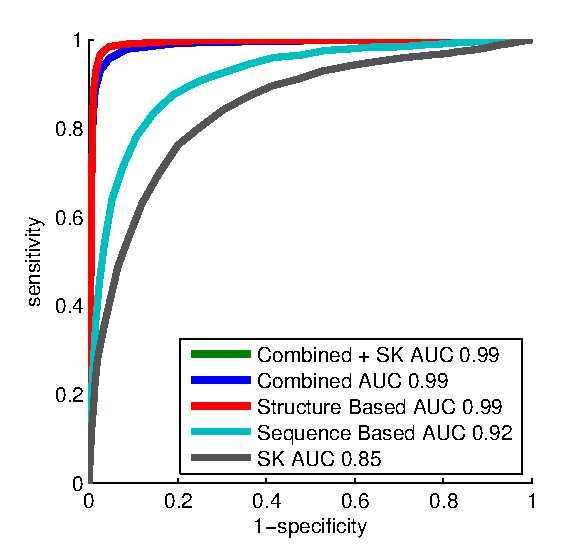
\includegraphics[width=\textwidth]{Figures/vq/SCOP_ROC/all_alpha_ROC}
                \caption{Alll $\alpha$}
                \label{fig:ocS1A}
        \end{subfigure}%
        \quad
	\begin{subfigure}[b]{0.23\textwidth}
                \centering
                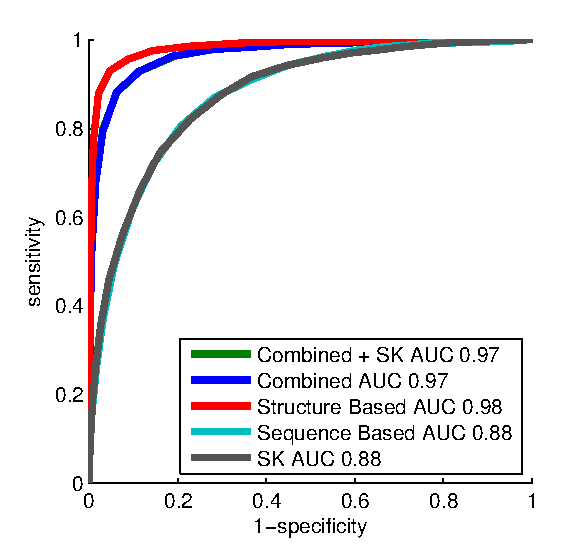
\includegraphics[width=\textwidth]{Figures/vq/SCOP_ROC/all_beta_ROC}
                \caption{All $\beta$}
                \label{fig:ocS1B}
        \end{subfigure}
	\quad
	\begin{subfigure}[b]{0.23\textwidth}
                \centering
                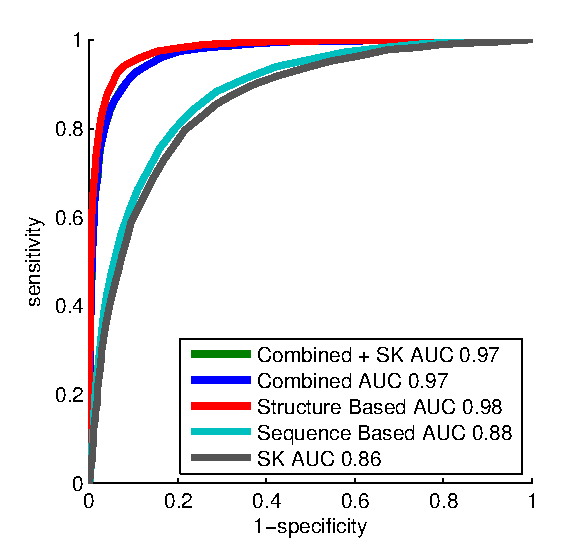
\includegraphics[width=\textwidth]{Figures/vq/SCOP_ROC/alpha_div_beta_ROC}
                \caption{$\alpha$/\ $\beta$}
                \label{fig:ocS1A}
        \end{subfigure}%
        \quad
	\begin{subfigure}[b]{0.23\textwidth}
                \centering
                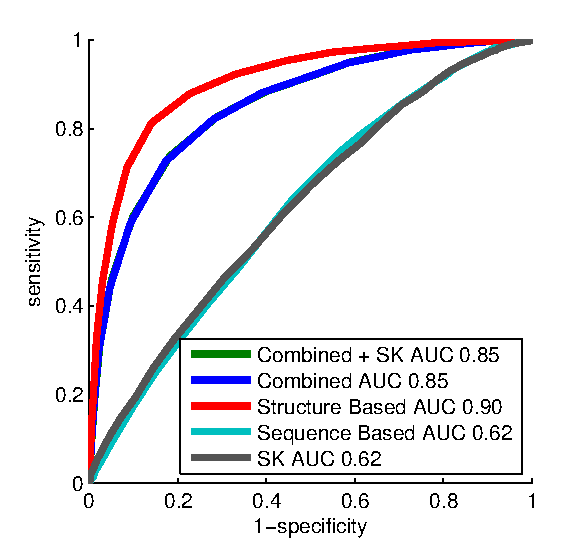
\includegraphics[width=\textwidth]{Figures/vq/SCOP_ROC/alpha_plus_beta_ROC}
                \caption{$\alpha$ + $\beta$}
                \label{fig:ocS1B}
        \end{subfigure}

\end{centering}
\caption[SCOP ROC curves]{SCOP ROC curves showing the performance of each combination of combined features and the string kernel when predicting each category of SCOP fold tested.}
\label{fig:SCOP_ROC}
\end{figure*}




%%%%%%%%%%%%%%%%%%%%%%
%%%%%%%%%%%%%%%%%%%%%%

%\begin{figure*}[t!]
%\begin{centering}
%	\begin{subfigure}[b]{0.35\textwidth}
%                \centering
%                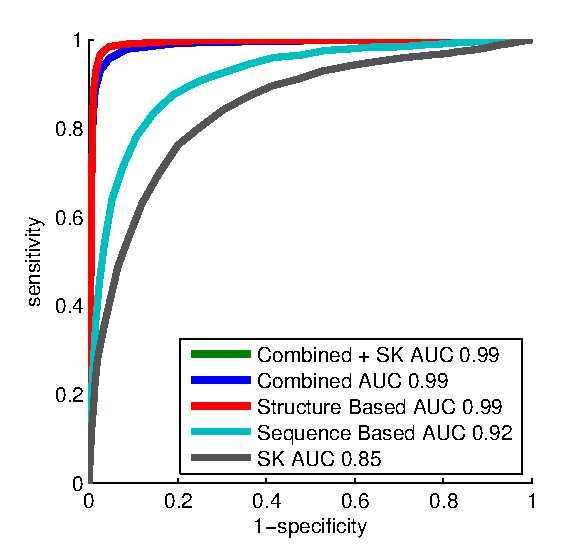
\includegraphics[width=\textwidth]{Figures/vq/SCOP_ROC/all_alpha_ROC}
%                \caption{Alll $\alpha$}
%                \label{fig:ocS1A}
%        \end{subfigure}%
%        \quad
%        \quad
%        \quad
%	\begin{subfigure}[b]{0.35\textwidth}
%                \centering
%                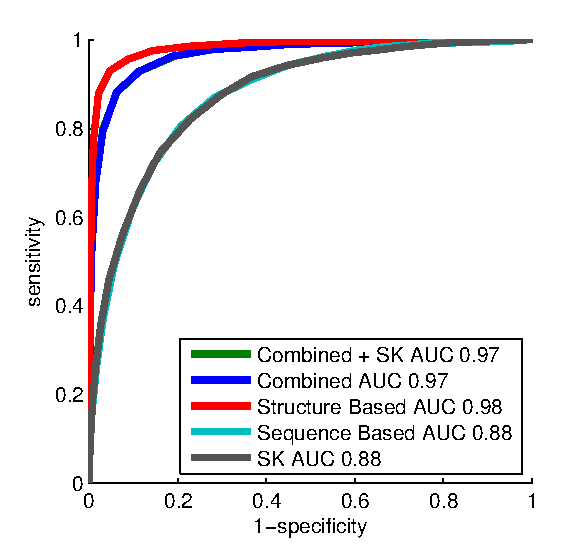
\includegraphics[width=\textwidth]{Figures/vq/SCOP_ROC/all_beta_ROC}
%                \caption{All $\beta$}
%                \label{fig:ocS1B}
%        \end{subfigure}
%
%	\begin{subfigure}[b]{0.35\textwidth}
%                \centering
%                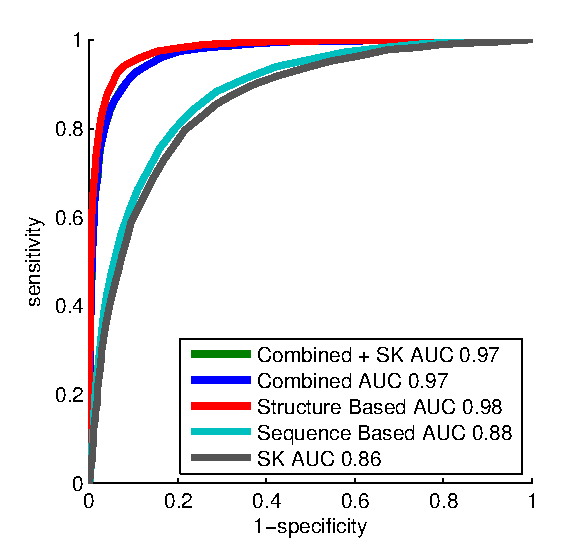
\includegraphics[width=\textwidth]{Figures/vq/SCOP_ROC/alpha_div_beta_ROC}
%                \caption{$\alpha$/\ $\beta$}
%                \label{fig:ocS1A}
%        \end{subfigure}%
%        \quad
%        \quad
%        \quad
%	\begin{subfigure}[b]{0.35\textwidth}
%                \centering
%                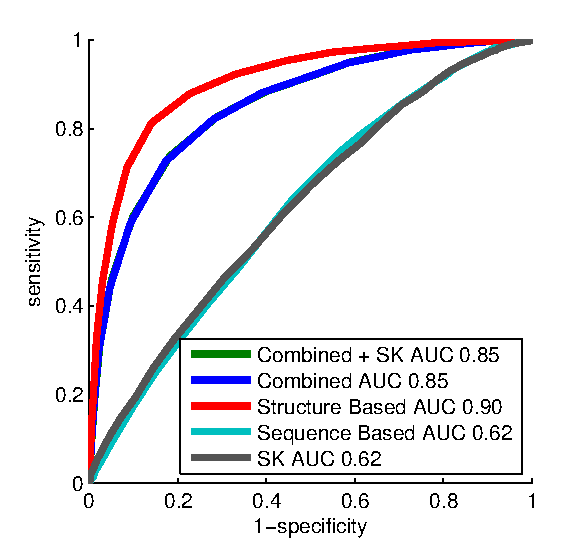
\includegraphics[width=\textwidth]{Figures/vq/SCOP_ROC/alpha_plus_beta_ROC}
%                \caption{$\alpha$ + $\beta$}
%                \label{fig:ocS1B}
%        \end{subfigure}
%
%\end{centering}
%\caption[SCOP ROC Curves]{SCOP ROC Curves showing the performance of each combination of combined features and the string kernel when predicting each category of SCOP fold tested.}
%\label{fig:SCOP_ROC}
%\end{figure*}

%%%%%%%%%%%%%%%%%%%%%%
%%%%%%%%%%%%%%%%%%%%%%
%%%%%%%%%%%%%%%%%%%%%%
%%%%%%%%%%%%%%%%%%%%%%

%%%%%%%%%%%%%%%%%%%%%%
%%%%%%%%%%%%%%%%%%%%%%
\subsubsection{Catalytic activity}
%%%%%%%%%%%%%%%%%%%%%%
%%%%%%%%%%%%%%%%%%%%%%

We obtained marginal improvements when combining sequence based properties, achieving a $AUC^{\bf{w}}$ of $0.776$ compared to an $AUC^{\bf{w}}$ of $0.742$ for VSL2B.

%% Figure
%%%%%%%%%%%%%%%%%%%%%%
%%%%%%%%%%%%%%%%%%%%%%
%%%%%%%%%%%%%%%%%%%%%%
%%%%%%%%%%%%%%%%%%%%%%

\begin{figure*}[t!]
\begin{centering}
	\begin{subfigure}[b]{0.25\textwidth}
                \centering
                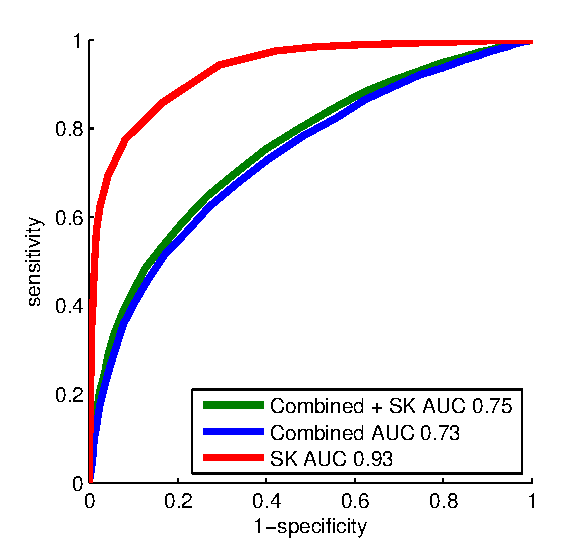
\includegraphics[width=\textwidth]{Figures/vq/GO_SC_ROC/hydrolase_activity_ROC}
                \caption{hydrolase activity}
                \label{fig:hydrolase_activity_ROC}
        \end{subfigure}%
        \quad
	\begin{subfigure}[b]{0.25\textwidth}
                \centering
                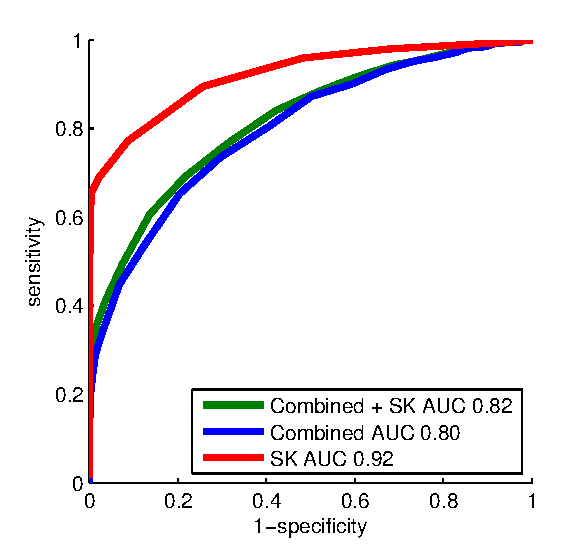
\includegraphics[width=\textwidth]{Figures/vq/GO_SC_ROC/isomerase_activity_ROC}
                \caption{isomerase activity}
                \label{fig:isomerase_activity_ROC}
        \end{subfigure}
        \quad
	\begin{subfigure}[b]{0.25\textwidth}
                \centering
                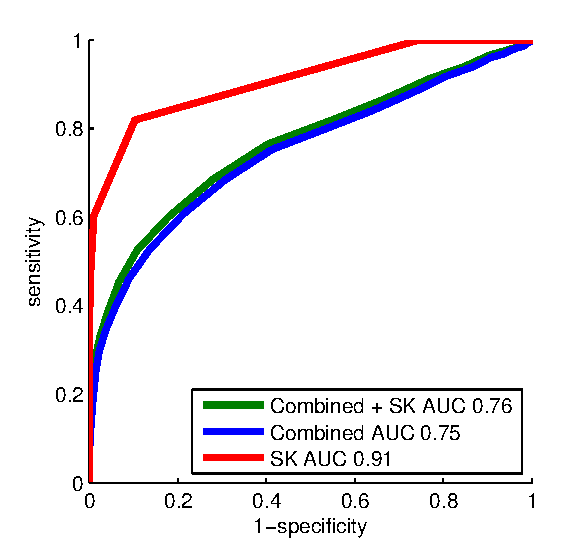
\includegraphics[width=\textwidth]{Figures/vq/GO_SC_ROC/ligase_activity_ROC}
                \caption{ligase activity}
                \label{fig:ligase_activity_ROC}
        \end{subfigure}

	\begin{subfigure}[b]{0.25\textwidth}
                \centering
                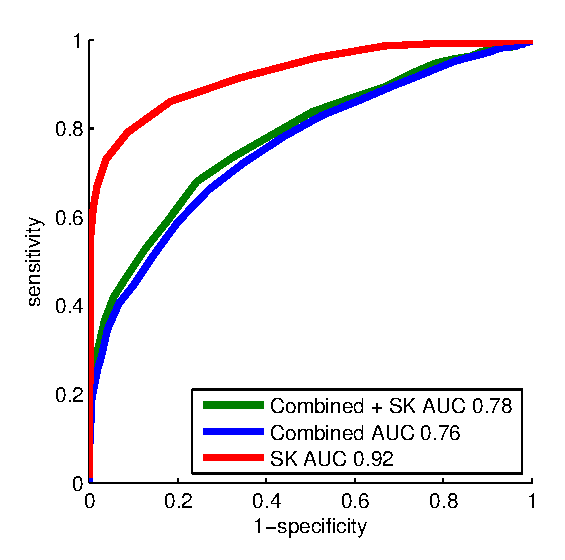
\includegraphics[width=\textwidth]{Figures/vq/GO_SC_ROC/lyase_activity_ROC}
                \caption{lyase activity}
                \label{fig:lyase_activity_ROC}
        \end{subfigure}%
        \quad
	\begin{subfigure}[b]{0.25\textwidth}
                \centering
                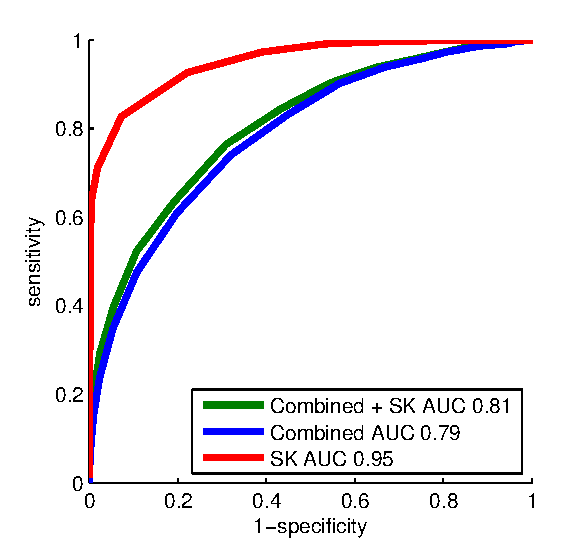
\includegraphics[width=\textwidth]{Figures/vq/GO_SC_ROC/oxidoreductase_activity_ROC}
                \caption{oxidoreductase activity}
                \label{fig:oxidoreductase_activity_ROC}
        \end{subfigure}
        \quad
	\begin{subfigure}[b]{0.25\textwidth}
                \centering
                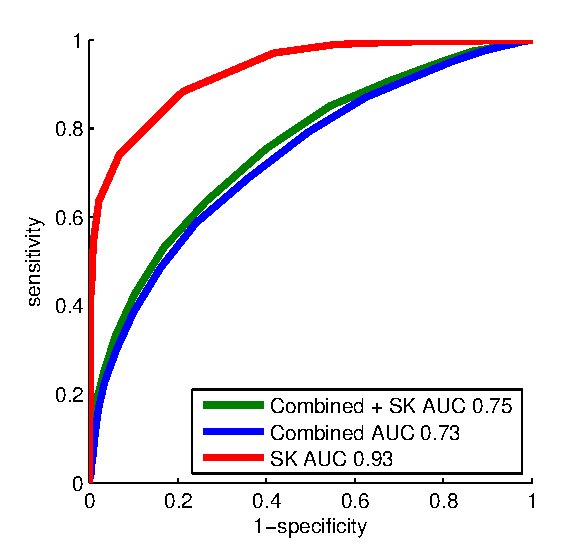
\includegraphics[width=\textwidth]{Figures/vq/GO_SC_ROC/transferase_activity_ROC}
                \caption{transferase activity}
                \label{fig:transferase_activity_ROC}
        \end{subfigure}

\end{centering}
\caption[``catalytic activity" subclass ROC curves]{ROC curves when showing the performance of each combination of combined features and the string kernel when predicting each subclass of ``catalytic activity".}
\label{fig:GO_SC_ROC}
\end{figure*}

%%%%%%%%%%%%%%%%%%%%%%
%%%%%%%%%%%%%%%%%%%%%%
%%%%%%%%%%%%%%%%%%%%%%
%%%%%%%%%%%%%%%%%%%%%%
\subsubsection{Catalytic activity subclass}

The most marked improvement in performance obtained by the combined kernel was when predicting catalytic activity subclass, achieving a $AUC^{\bf{w}}$ of $0.767$ compared to the highest $AUC^{\bf{w}}$ obtained by an individual sequence property of $0.659$ (predicted B-factors).

\subsection{String kernel performance}

We found that the string kernel outperformed sequence based properties in both the task of predicting catalytic activity and its subclass ($AUC^{\bf{w}}$ of $0.857$ and $0.930$) respectively.  On the other hand, the string kernel did not show superior performance when predicting SCOP fold, only obtaining a $AUC^{\bf{w}}$ of $0.794$ compared to an $AUC^{\bf{w}}$ of $0.961$ obtained by the combined structure kernel.

\subsection{Optimal parameter values}

\subsubsection{SCOP fold}
We found that structure-based properties consistently preferred large numbers of centroids, obtaining maximum $AUC$ at $m=4,096$ for all structure-based properties and all classification tasks.  Optimal window sizes were 8 or 16 amino acids for all SCOP folds besides $\alpha + \beta$ which favored wider window size, obtaining a maximum $AUC$ at $n=32$ for all folds.

Sequence-based properties were less consistent in the optimal values of $m$ and $n$, covering a range of values for each feature and SCOP fold.

\subsubsection{Catalytic activity}
There was very little variation in preferred values of $m$ when predicting catalytic activity with all features aside from predicted hydrophobicity obtaining maximum $AUC$ values at $m=256$.  There was much more variation in preferred window sizes with hydrophobicity obtaining smallest optimal window size of $2$, and B-factors and PDB Disorder preferring longer window sizes ($n=32$).

\subsubsection{Catalytic activity subclass}
Sequence based properties were much more consistent in the values of $m$ and $n$ preferred when predicting catalytic activity subclass, almost always preferring large values of $m$ ($4,096$)

\subsection{Comparing $\bf{AUC}$ and $\bf{SNR}$}

\Cref{fig:vq_snr} shows a scatterplot of $SNR$ and $AUC^{\mathbf{w}}$ values. We found that derived backbone angles obtained the lowest $SNR$ values.  Similarly, properties that obtained low $AUC^{\mathbf{w}}$ values seemed to have a higher range of SNR values.  Although backbone angles, as a class, obtained lower values of $SNR$, these values did not seem to correlate with higher $AUC$ values; and we found very little correlation with $SNR$ obtained at particular values of $AUC$ for this class of features \Cref{tab:snrcorr}, although they were the only property class to obtain a positive correlation between $SNR$ and $AUC$. The opposite was the case for VSL2B based disorder predictions and predicted secondary structure.  These features, which obtained the worst performance when predicting SCOP fold had the strongest negative correlation between $SNR$ and $AUC$.  While the trend of positive correlation (although weak) between $SNR$ and $AUC$ was observed for derived backbone angles, the overall trend for other features went against this trend.

\begin{figure*}[h!]
\begin{centering}
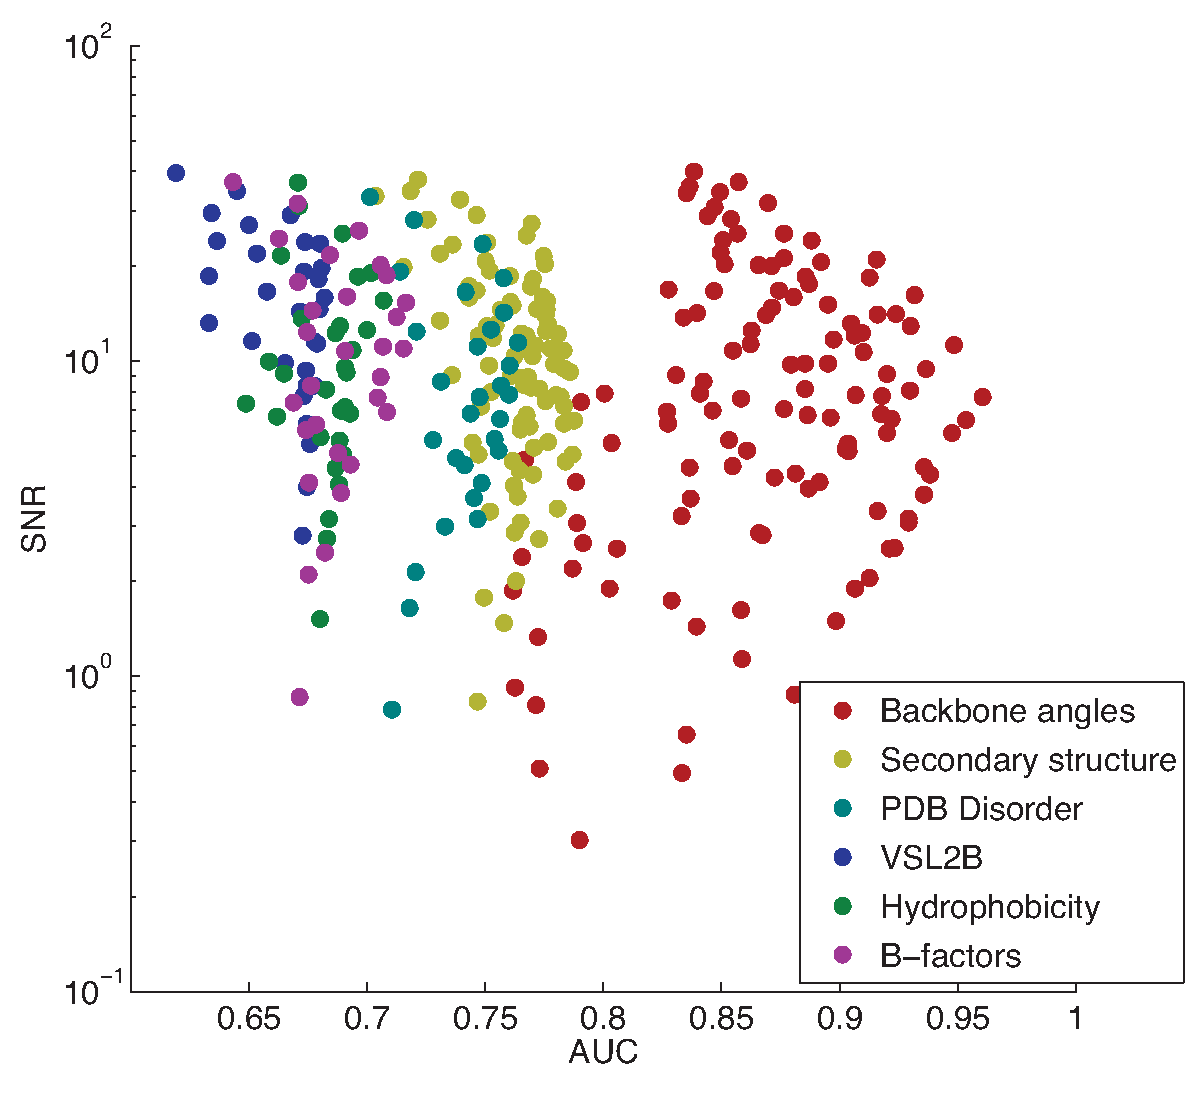
\includegraphics[width=.65\linewidth]{Figures/vq/SCOP_SNR_AUC}
\end{centering}
\caption[Comparison of SNR and AUC]{Comparison of $AUC$ and $SNR$.  For each feature type obtained SNR values were plotted as a function of $AUC^{\mathbf{w}}$ values for the prediction of SCOP fold.}
\label{fig:vq_snr}
\end{figure*}

%Table
%%%%%%%%%%%%%%%%%%%%%
%%%%%%%%%%%%%%%%%%%%%%
\begin{table}[h]
\centering
	\begin{tabular}{|l|r|}

		\hline		
		Property Class & \shortstack{Correlation \\Coefficient} \\
	
		\hline
		Backbone angles & $0.07$\\
		Secondary structure & $-0.52$\\
		PDB Disorder & $-0.21$\\
		VSL2B & $-0.58$\\
		Hydro & $-0.07$\\
		B-Factor & $-0.21$\\
		
		\hline    
	\end{tabular}

 \caption[Correlation between $AUC$ and $SNR$]{The correlation between $SNR$ and $AUC^{\mathbf{w}}$ for various properties. }
\label{tab:snrcorr}
\end{table}
%%%%%%%%%%%%%%%%%%%%%
%%%%%%%%%%%%%%%%%%%%%


\subsection{Reduced redundancy data set}


\begin{figure*}[h!]
\begin{centering}

\includegraphics[width=.55\textwidth]{Figures/VQ/NR40CA}
\par\end{centering}
\caption[NR40 catalytic activity results]{ROC curves obtained when combining the string kernel with sequence properties (green line), combining all sequence properties (blue curve), and the string kernel (red curve) when predicting catalytic activity on the $40\%$ non redundant data set of proteins.}
\label{fig:NR40}
\end{figure*}



We also generated a reduced redundancy data set of proteins with GO annotations in which the maximum pairwise sequence identity output by BLAST between any two sequences was $40\%$.  This non-redundant $40\%$ data (NR40) set was generated to simulate the performance of each property when, for a given query protein, there is no sequence that is both annotated and of a reasonable level of sequence similarity.

We found that although the string kernel outperformed sequence properties when predicting catalytic activity, the combined sequence property kernel outperformed the string kernel when predicting catalytic activity.  As shown by \Cref{fig:NR40} the combined sequence property kernel obtains slightly better performance than the string kernel, obtaining an $AUC$ of $0.78$ compared to $0.73$ respectively.  Interestingly, the combined string kernel and sequence property kernel did not achieve improved performance, obtaining the same $AUC$ as the combined sequence property kernel ($0.78$).  This is similar to the performance of the same set of features when applied to the non reduced redundancy data set, although in that case the combine string kernel and sequence property kernel grouped with the sequence property features.

When predicting catalytic activity subclass we observed similar results as on the unfiltered data set; the string kernel obtained higher $AUC$ values than both the sequence property kernel and the combined string kernel and sequence property kernel for all tested subclasses of catalytic activity.
%%%%%%%%%%%%%%%%%%%%%%
%%%%%%%%%%%%%%%%%%%%%%
%\afterpage{
%\begin{figure*}[t!htpb]
%\begin{centering}
%
%	\begin{subfigure}[b]{0.75\textwidth}
%                \centering
%                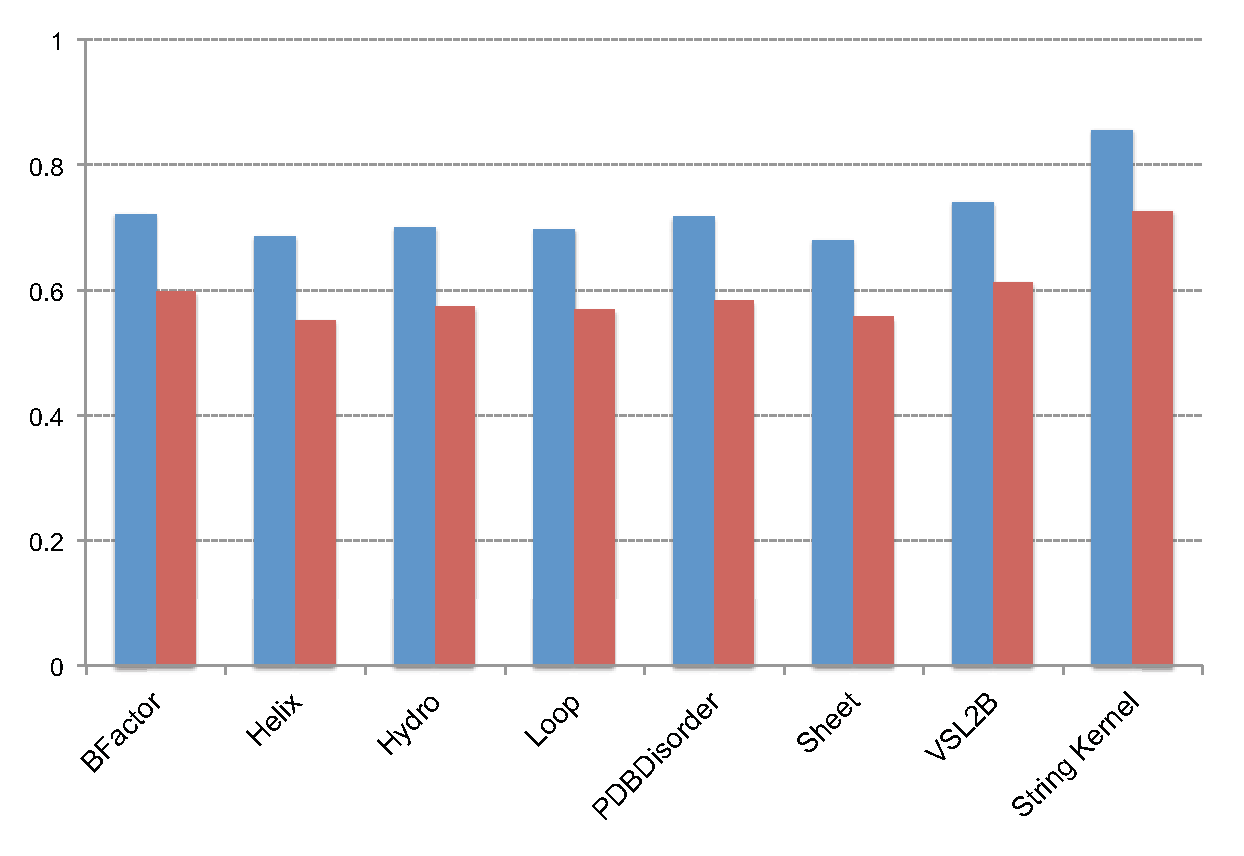
\includegraphics[width=\textwidth]{Figures/vq/count_kernel/GO_Enzyme_Bar}
%                \caption{Catalytic activity}
%                \label{fig:vqresults1B}
%        \end{subfigure}%
%\quad
%	\begin{subfigure}[b]{0.75\textwidth}
%                \centering
%                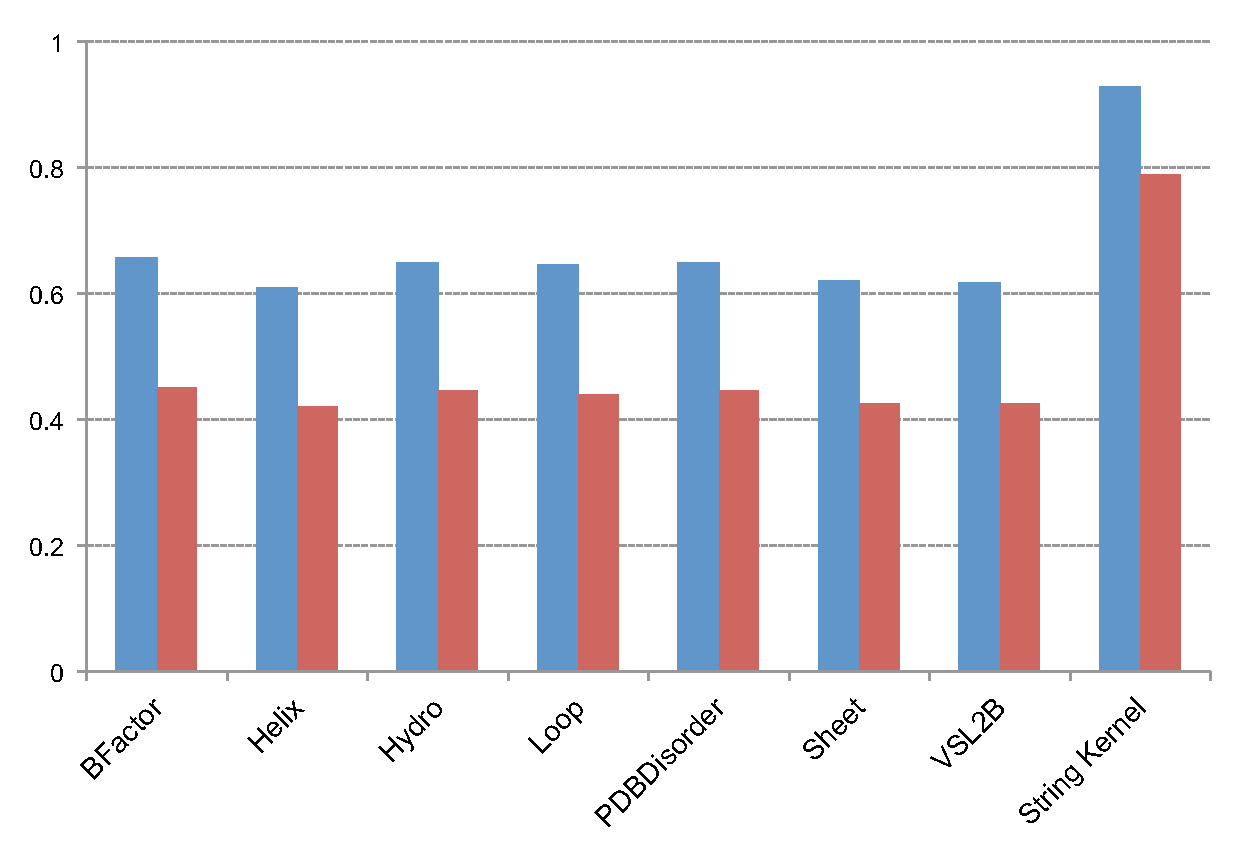
\includegraphics[width=\textwidth]{Figures/vq/count_kernel/GO_SC_Bar}
%                \caption{Catalytic activity subclass}
%                \label{fig:vqresults1C}
%        \end{subfigure}%
%
%
%\par\end{centering}
%\caption[Count kernel individual feature performance]{A bar chart showing the $AUC$ (blue) and $F_{\max}$ (red) performance of individual features in the task of GO function prediction.  Only the best performing combinations of $m$ and $n$ for an individual feature according to $AUC$ or $F_{\max}$ are reported.  Results are shown for the task of predicting  ``catalytic activity" GO term (\Cref{fig:vqresults1B}), and ``catalytic activity" subclass (\Cref{fig:vqresults1C}).  }
%\label{fig:vqresults1}
%\end{figure*}
%}
%%%%%%%%%%%%%%%%%%%%%%
%%%%%%%%%%%%%%%%%%%%%%
%%%%%%%%%%%%%%%%%%%%%%
%%%%%%%%%%%%%%%%%%%%%%
%\begin{figure*}[h!]
%\begin{centering}
%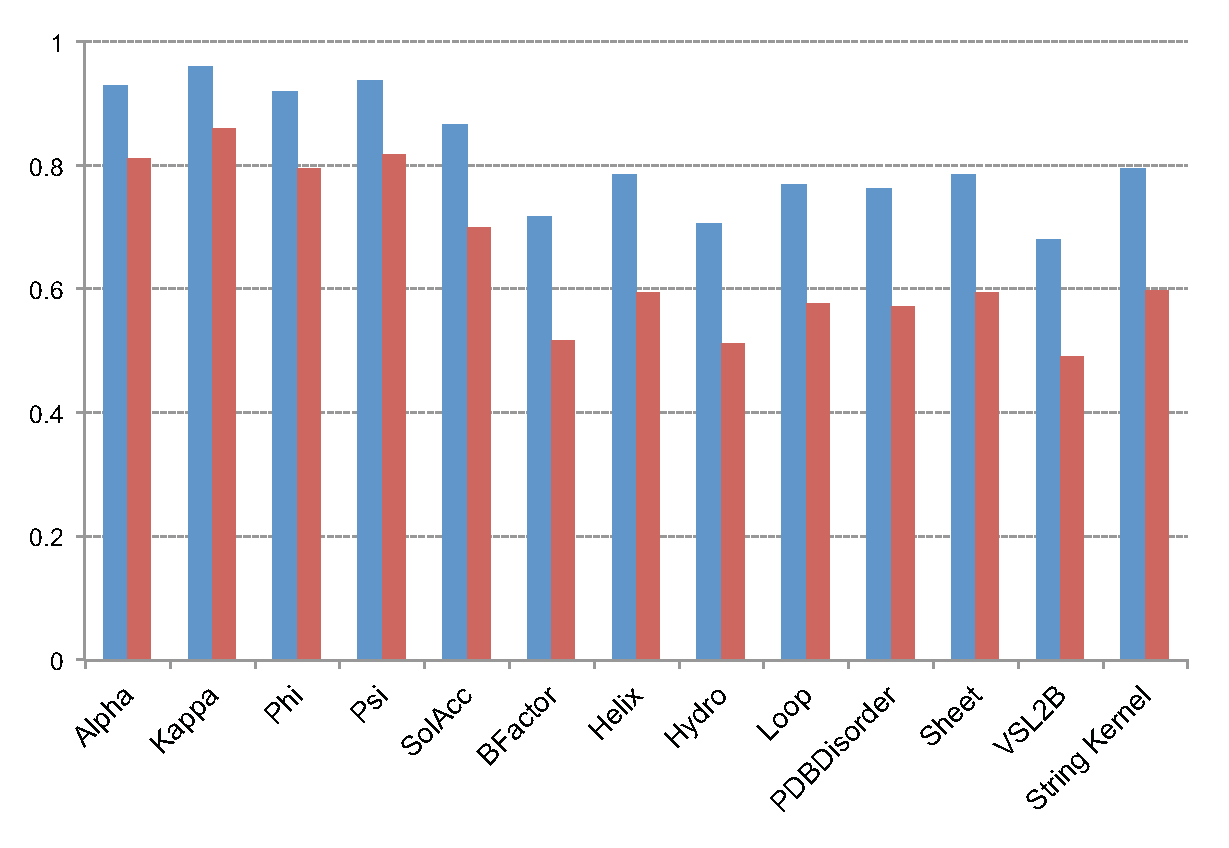
\includegraphics[width=.75\textwidth]{Figures/vq/count_kernel/SCOP_Bar}
%\par\end{centering}
%\caption[Count based kernel performance predicting SCOP fold]{A bar chart showing the $AUC$ (blue) and $F_{\max}$ (red) performance of individual features. Only the best performing combinations of $m$ and $n$ for an individual feature according to $AUC$ or $F_{\max}$ are reported. }
%\label{fig:vqscopcount}
%\end{figure*}
%%%%%%%%%%%%%%%%%%%%%%
%%%%%%%%%%%%%%%%%%%%%%


%%%%%%%%%%%%%%%%%%%%%%%
%%%%%%%%%%%%%%%%%%%%%%%
%\subsection{Agreement of $AUC$ and $F_{\max}$}
%%%%%%%%%%%%%%%%%%%%%%%
%%%%%%%%%%%%%%%%%%%%%%%
%
%Looking at \Cref{tab:vqgostandardperformance,tab:vqscopstandardperformance} we found strong agreement in the values of $m$ and $n$ at which each feature type achieved its maximum $AUC$ and $F_{\max}$ values for the count based kernel, especially for the prediction of SCOP fold and ``catalytic activity" subclass.  While agreement wasn't as strong for the prediction of ``catalytic activity," differences in optimal $m$ and $n$ values were not drastic; the most notable of which were those determined for the hydrophobicity property feature where $AUC$ found that $m=4096, n=2$ was optimal whereas $F_{\max}$ found that $m=256, n=32$ was optimal.  
%
%%There was noticeably less agreement between optimal $m$ and $n$ values designated by $AUC$ and $F_{\max}$ when looking at the similarity augmented count kernel, with the $F_{\max}$ value seeming to favor smaller numbers of centroids for structure based features.  While there is little agreement between these metrics for the similarity augmented count kernel this may be due to the poor overall performance of this kernel.
%%
%%Although the sample size for determining agreement in optimal $m$ and $n$ values is smaller for the additive kernel because it was only fully tested on the hydrophobicity sequence property, there are multiple alpha values at which optimal $m$ and $n$ values can be compared.